\chapter{Methods}
%just some stuff for the sphere in the cube graphic
\tikzset{
    MyPersp/.style={scale=1.8,x={(-0.8cm,-0.4cm)},y={(0.8cm,-0.4cm)},
    z={(0cm,1cm)}},
    MyPoints/.style={fill=white,draw=black,thick}
    }
    
This section has the purpose to give an overview over all changes in the project which occurred during this bachelor thesis. These changes include some small improvements of the application as well as how to draw a sphere cell. First minor changes are briefly described, deeper in this section the more effortful changes are explained. 

\section{Lambda multipliers}
In the project there were several places, where the multipliers $\lambda_{vol}$ and $\lambda_{sur}$ are calculated, but they are only set when a cell is initialized. The multiplier for the volume is set a second time in the necrosis event, if the program models that a cell dies. \newline
There are two additional multipliers, for the surface and volume constraints, saved in within each cell object. Since we are not using these values in the program and they do not influence or set the $\lambda_{vol}$ or $\lambda_{sur}$ which \ac{CC3D} uses, these two values are deleted. Moreover, in one place there were methods to calculate the lambda values. Since these methods are not used in the project and they had a multiplier itself to calculate the multiplier for the specific part of the effective energy, they are deleted as well. 

In the project the multipliers $\lambda_{vol}$ and $\lambda_{sur}$ are now set each time when a cell is initialized. A second time the multiplier $\lambda_{vol}$ is set, is if necrosis takes place. Because now the unnecessary methods and values for the multipliers values are removed, no confusion about which constraint values in the program are used will come up.

\section{Abstract methods}
In the program, in several classes there were methods, which are not used. These methods are not used in the class, in which they are written, due to polymorphism. They are used in classes, which inherit from the class where they are written. Polymorphism is a method out of \ac{OOP}. Another technique out of \ac{OOP} is the use of abstract classes and abstract methods. To explain polymorphism, abstract classes or abstract methods in detail, would take too much space out of this bachelor thesis. Thus, the change in the program is explained in the following.

In the project there a several classes which inherit from each other. In these classes there were the same methods implemented. Since it is not required that all classes have to have the same methods, these are redundant methods, as long as they do not differ in their functionality. For such methods it is possible to declare them as an abstract method. An abstract method contains only the method construct, but no functionality. Due to polymorphism the class in which such an abstract method is implemented is used to call this method. \newline
In python there is a library 'abc'. With this library it is possible to declare an abstract method. To do so every class with one or more abstract methods needs to initialize a special class variable. With this variable python is able to recognize that there are abstract methods included.

\begin{lstlisting}[language=Python, caption = The initialization of a class variable which is required by python in order to detect abstract methods and abstract classes.]
class ModelConfig(object):
    __metaclass__ = ABCMeta
\end{lstlisting}

The listing above displays how the class variable has to be initialized in order that abstract methods are recognized. If a class has at least one abstract method, it is an abstract class. In python abstract classes can include implemented methods as well as abstract methods.

\begin{lstlisting}[language=Python, caption = Declaration of an abstract method.]
    @abstractmethod
    def _createExecConfig(self):
        pass
\end{lstlisting}

The listing above is an example of an abstract method in python. Using abstract methods creates more structure and clarity within the project. Therefore, the abstract declarations in this project created a much better clarity of the structure of the project and of the methods, which were used in the classes.

\section{Calculation steps until urination}
To simulate the urination in the program it was checked if the current calculation step is larger than 250 and a factor of 125. Because every 250 \ac{MCS} the volume- and arrangement fitness functions are calculated and no other events in the simulation take place, the urination was simulated every 12 hours. The check if the current \ac{MCS} is a factor of 125 happens with the modulo operator. Thus, the current calculation step is divided by 125 and if the result, as a whole number, is 0 it is a factor. \newline
The check when the urination event takes place is modified. The urination event now takes place if the current calculation step is larger than 250 and if the current \ac{MCS} modulo 125 equals 1. Therefore, the urination event is used every 6 hours, at \ac{MCS} 376, 501, 626, 751, etc..

\section{Area of stem cells on the basal membrane}\label{sec:AmountStemCellsBasalMembrane}
In an earlier version of the project it was evidenced that around 12\% of the area of the basal membrane are required to be filled with stem cells in order to have an optimal proliferation during the morphogenesis of the cells \cite{Torelli2017}.
In the project the calculation of the amount of stem cells for two dimensions were correct but without an mathematical evidence. \newline
Since the y-axis is negligible in the calculation of an area, the calculation for two dimensions considers the x-axis and the calculation for three dimensions considers the x- and z-axis. Therefore, in two dimensions the area of the stem cells should be calculated by using the cell diameter. An illustration therefor is displayed in figure \ref{tikz:AreaIn2D}. For three dimensions it is possible to calculate the area of a circle with the formula $A = \pi \cdot r^{2}$, because a sphere in 2D is a circle, and use this calculation to further determine the amount of stem cells on the basal membrane. An example for the basal membrane and a stem cell in three dimensions is displayed in figure \ref{tikz:AreaIn3D}. 

\begin{figure}[h]
\begin{center}
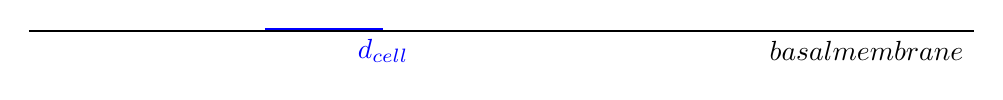
\begin{tikzpicture}[scale=3]
%%draw the edges of the cube
\draw[black,thick] (-2,0) -- (2,0)node[anchor=north east]{$basal membrane$};
\draw[blue,thick] (-1,.01) -- (-0.5,.01)node[anchor=north]{$d_{cell}$};
\end{tikzpicture}
\caption{Considered area to spread the stem cells in 2D with an example of one stem cell placed on the basal membrane. Because only the x-axis is displayed we need to calculate the diameter of a cell.}
\label{tikz:AreaIn2D}
\end{center}
\end{figure}


\begin{figure}[h]
\begin{center}
\begin{tikzpicture}[MyPersp,font=\large]
%%draw the edges of the cube
%\draw[pattern=north west lines, pattern color=blue] (0,0) rectangle (2,4);
\draw[pattern=north west lines, pattern color=gray] (0,0,0) -- (0,2.25,0) -- (3.25,2.25,0) -- (3.25,0,0) -- cycle;
\fill[blue] (1,1.75)   circle[radius=0.125];
 
\end{tikzpicture}
\caption{Considered area to spread the stem cells in 3D with an example of one stem cell placed on the basal membrane. The hatched area displays the basal membrane and the circle represents one stem cell. This stem cell is a circle, because in the calculation of the amount of stem cells the y-axis is negligible.}
\label{tikz:AreaIn3D}
\end{center}
\end{figure}


With the following two equations it is possible to calculate the amount of stem cells in two dimensions. $A_{stem cells}$ refers to the area which can be used for stem cells. Therefore, it is 12\% of the basal membrane. C is a constant, which describes 12\% of an object. Thus, $c=0.12$.

\begin{equation}\label{eq:Area12-2D}
A_{stem cells} = xLength \cdot c
\end{equation}
\begin{equation}\label{eq:AmounStemCell2D}
Amount_{StemCells} = \dfrac{A_{stem cells}}{d_{cell}} 
\end{equation}
Equation \ref{eq:Area12-2D} ensures that only 12\% of the given area is used. Formula \ref{eq:AmounStemCell2D} then calculates the amount of stem cells on this given area. Because the result of the calculation is often not a whole number, the result is checked if the first decimal digit is larger or equal than 5 and then it is rounded up or casted, i.e. the decimal digits are cut off.

\begin{table}
\centering
\caption{Possible approximation error by not rounding the result of equation \ref{eq:AmounStemCell2D}. The first column describes the length of the basal membrane, the values are  in \SI{}{\micro\metre}. In the second column the result of equation \ref{eq:AmounStemCell2D} is displayed. In the third column the result of the second column is rounded up in the first row. In the second row this result is casted. The fourth column displays how much space the stem cells, in \SI{}{\micro\metre}, of the rounded or casted result of eqataion \ref{eq:AmounStemCell2D} require. The last column displays the physical space required in percentage to the basal membrane.}
\renewcommand{\arraystretch}{1.5}
	\begin{tabularx}{\textwidth}{X||X||X||X||X}
		xLength of the basal membrane & Result of equation \ref{eq:AmounStemCell2D} & Amount of stem cells & Area used of stem cells  in \SI{}{\micro\metre} & relative used area  \\
		\hline
		200 & $\sim 2.66$ & 3 & 27 & 13.5\% \\
		
		200 & $\sim 2.66$ & 2 & 18 & 9\% 

	\end{tabularx}
	\label{tbl:Approximation error}
\end{table}

As table \ref{tbl:Approximation error} displays, it is important to round the result. Otherwise there would be an approximation error and as a result a calculation error. \newline
For three dimensions the equation \ref{eq:Area12-2D} has to be extended, because the z-axis is now also considered in the calculation of the amount of stem cells on the basal membrane. An illustration therefor is figure \ref{tikz:AreaIn3D}. Equation \ref{eq:AmounStemCell2D} has to be modified, because now the area of an circle, instead of the diameter, is used for the calculation. Therefore, the equations to calculate the amount of stem in three dimensions are:
\begin{equation}\label{eq:Area12-3D}
A_{stem cells} = (xLength \cdot zLength) \cdot c
\end{equation}
\begin{equation}\label{eq:AmounStemCell3D}
Amount_{StemCells} = \dfrac{A_{stem cells}}{\pi \cdot r^{2}} 
\end{equation}
The result of formula \ref{eq:AmounStemCell3D} has to be rounded as well, otherwise the program would include rounding errors. 
These calculations are now included in the program.

%In the following listing the calculation for the amount of stem cells on the basal membrane is shown. The calculation uses the equations of this subsection. If the program has to round up the result. The result will be increased by 1 and then it will be casted. This functionality has and mathematical evidence, which is useful as it allows the program to be more resistant against errors.
%
%\begin{lstlisting}[language=Python, caption= new calculation of the amount of stem cells on the basal membrane with a mathematical evidence]
%    def _initCells(self, steppable):
%...
%        c = 0.12 # the area used of stem cells in percentage
%        cellDiameter = self.cellTypes[2].getAvgDiameter()  # cell diameter is of type float
%        
%        if self.execConfig.dimensions == 2:
%            noStemCells = int(self.execConfig.xLength * c / cellDiameter)
%        else:
%            noStemCells = ((self.execConfig.xLength * self.execConfig.zLength) * c) / (PI * (cellDiameter / 2.) ** 2)
%
%        if noStemCells % 1 > 0.5:
%            noStemCells += 1
%
%        noStemCells = int(noStemCells)
%...
%\end{lstlisting}


\section{Target volume and target surface after mitosis}
Mitosis of the cell is simulated by \ac{CC3D}. In the simulation mitosis is simulated as the following: one cell splits into two cells. The cell which splits dies and then two new cells out of the died cell are created. \newline
In the program we specify and check if and when a cell splits. \ac{CC3D} decides where the cell splits and calculates the volume and surface of the two new cells. In our program we calculate and set attributes of the new cells, e.g. the target volume or the target surface. \newline 
The target volume is calculated by dividing the target volume of the cell before mitosis by 2. This value is applied for both new created cells. The problem with this technique is that it is possible that the cell might not split in the middle. In the case of mitosis, setting the target volume of the two created cells without the knowledge of the volume is a source of error. Because the target volume of the two new cells are set without considering the current volume of the cell, it occurred that one of the new cells, after mitosis, had a target volume which was smaller than the current volume. \newline
After mitosis both cells are initialized. Thus, the target volume and target surface is calculated and set. After the initialization of the cells is done, the target volume of the new cells is set to the target volume divided by 2 of the cell before mitosis. \newline
Because the target volume is calculated out of the current volume of the cell during the initialization process, the calculation of the target volume is removed out of the mitosis event. Now the target volume and surface after mitosis is set only during the initialization process of the new cells. \newline
With this change of the program the case that some cells have a smaller target volume than the current volume disappeared. In the program, the target volume and target surface after mitosis is calculated and set dependent on the of \ac{CC3D} given volume.



\section{Approximation Error}
Because the project includes conversions from \SI{}{\micro\metre} into voxels and the amount of pixels, e.g. for the surface of a cell, has to be set as data type integer, i.e. a whole number, it is possible that in some places in the program there are approximation errors. In the project, the values of unit \SI{}{\micro\metre} are saved with the data type float, i.e. a number with decimal digits. To set these values as a whole number the values are casted into the data type integer. 

Whenever a conversion from \SI{}{\micro\metre} into voxels is done the complete calculation is calculated with decimal digits. After the calculation is done it is verified if the first decimal digit is larger or equal to 5. If this condition is true the result is increased by 1, otherwise not. As a last step the result is casted. This technique has the advantage that calculation errors due to casting are removed, because the cast is the very last step. It is possible that in the program still include some rounding errors, but these can not be removed because \ac{CC3D} requires the amount of voxels as a whole number and the calculation is with decimal digits. \newline
In the function displayed below, the cast and the rounding of the result are done in the last step of the calculation.

\begin{lstlisting}[language=Python, caption = Function to calculate the volume of a sphere in voxels out of a given physical volume. First out of the given physical volume the radius is calculated. Then it is converted into the voxel unit. Next\, the volume of the voxel sphere is calculated and as last step\, the result is rounded and casted.]
   def calcVoxelVolumeFromVolume(self, volume):
        r = (3 * volume / (4.0 * PI)) ** (1.0 / 3.0)  # Radius of a sphere with known volume.
        rDimension = r * self.voxelDensity
        if self.dimensions == 2:
            return int(self.__truncate(PI * (rDimension ** 2)))  # Area of a circle.
        else:
            result = 4.0 / 3.0 * PI * (rDimension ** 3)
            if result % 1.0 >= 0.5:
                result += 1

            return int(result)
\end{lstlisting}

One use of the displayed function is to calculate the voxel volume out of the physical volume of a cell. In the simulation a minimum and a maximum volume for each cell type is calculated. These values are used in the calculation to determine if mitosis takes place or not. \newline
For the basal cell the minimum volume is \SI{381}{\micro\metre} and the maximal volume is \SI{523}{\micro\metre}. In table \ref{tbl:CellConstraints} at page \pageref{tbl:CellConstraints} the constraints of the different cell types in \SI{}{\micro\metre} are displayed. In the table \ref{tbl:Approximation error} three different possible calculations of the conversion of a volume in \SI{}{\micro\metre} into a volume in voxels are presented.

\begin{table}[h]
\centering
\caption{Three different ways to calculate the voxel volume out of a given physical volume. The first column describes the physical volume in \SI{}{\micro\metre}. In the second column the radius in \SI{}{\micro\metre} out of the volume is calculated. Next, the radius is used as it is, casted or rounded up. In the fourth column the exact result of the volume in voxel is presented and in the last column the rounded result of the voxel volume is displayed.}
\renewcommand{\arraystretch}{1.5}
	\begin{tabularx}{\textwidth}{X||X||X||X||X}
		Volume in \SI{}{\micro\metre} & radius in \SI{}{\micro\metre} & radius used in further calculation & not rounded result in vx & rounded result in vx  \\
		\hline
		381 & 4.49 & 4.497 & 1285.67 & 1286 \\
		
		381 & 4.49 & 4 & 904.77 & 905\\
		
		381 & 4.49 & 5 & 1767.15 & 1767\\

	\end{tabularx}
	\label{tbl:Approximation error}
\end{table}

In the table, the first row calculates the voxel volume as it is done in project right now. Thus, rounding and casting is the last step in the calculation. In the second raw the radius is calculated and casted. Then this casted radius is used for the further calculation. The third row calculates the radius and rounds it immediately. This rounded radius is then used for the further calculation. \newline
As the table displays, there is a significant difference in all three results. Because such a calculation is used to determine when a cell splits as well as it calculates the growth per \ac{MCS}, it influences the result of a simulation. Thus, it is important to round and cast the result as very last step in the calculation.




\section{Draw Sphere Cells}
Since a sphere as a cell is an approximation to a cell in the urothelium, it is a possible technique to draw and further simulate a cell as a sphere. \newline 
To be able to draw a sphere out of voxels it is required that a cuboid lays around the sphere, as it is displayed in \ref{tikz:SphereInCube}. The cuboid has to be at least as large as $2 \cdot radius$ of the sphere. In addition, the cuboid should not be larger than necessary, otherwise there would be unnecessary computable cost. The illustration in figure \ref{tikz:CuboidSphere} at page \pageref{tikz:CuboidSphere} display the perfect size of a square and a circle. These 2D objects are chosen to display the boundaries of a circle in a square as well as the boundaries would be in three dimensions.


To be able to draw a cell as a sphere, \ac{CC3D} has to allow the user to draw several different voxels in the simulation field, all containing to one cell. Since \ac{CC3D} allows the user to draw several pixels containing to one cell, a solution for this problem is possible.


\begin{figure}
\begin{center}
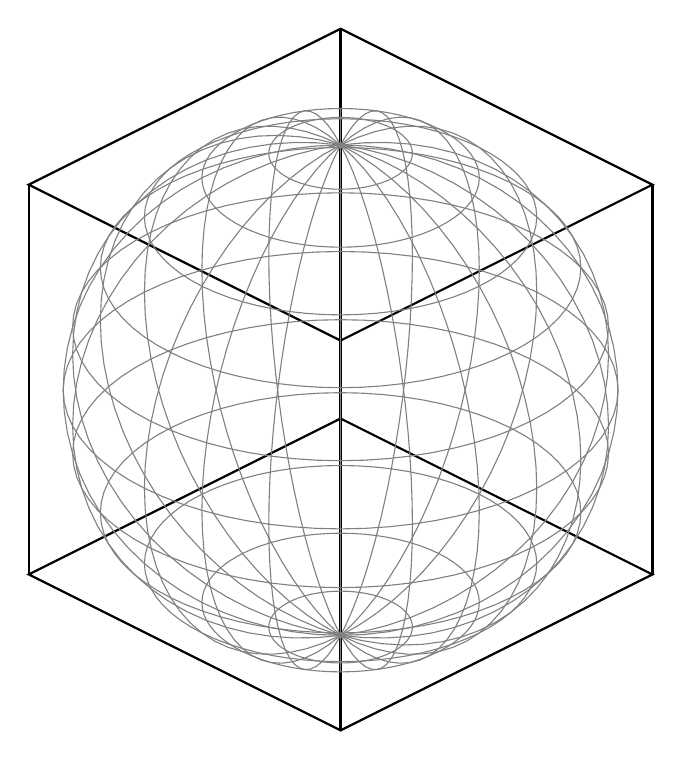
\begin{tikzpicture}[MyPersp,font=\large]%[scale=3]
%draw the three axis
%\draw[thick,->] (0,0,0) -- (3.0,0,0) node[anchor=north east]{$x$};
%\draw[thick,->] (0,0,0) -- (0,3.0,0) node[anchor=north west]{$y$};
%\draw[thick,->] (0,0,0) -- (0,0,3.0) node[anchor=south]{$z$};

\draw[black,thick] (0,0,0) -- (0,2.75,0) -- (2.75,2.75,0) -- (2.75,0,0) -- cycle;
\draw[black,thick] (0,0,2.75) -- (0,2.75,2.75) -- (2.75,2.75,2.75) -- (2.75,0,2.75) -- cycle;
%
%%draw the edges of the cube
\draw[black,thick] (0,0,0) -- (0,0,2.75);
\draw[black,thick] (0,2.75,0) -- (0,2.75,2.75);
\draw[black,thick] (2.75,0,0) -- (2.75,0,2.75);
\draw[black,thick] (2.75,2.75,0) -- (2.75,2.75,2.75);

\foreach \t in {0,15,...,150}% meridians
    {\draw[gray] ({1.73*cos(\t)+1.0},{1.73*sin(\t)+1.0},1.0)
        \foreach \rho in {5,10,...,360}
            {--({1.73*cos(\t)*cos(\rho)+1.0},
 			{1.73*sin(\t)*cos(\rho)+1.0},{1.73*sin(\rho)+1.0})}--cycle;
    }
\foreach \t in {-75,-60,...,75}% parallels
   {\draw[gray] ({1.73*cos(\t)+1.0},1.0,{1.73*sin(\t)+1.0})
        \foreach \rho in {5,10,...,360}
           {--({1.73*cos(\t)*cos(\rho)+1.0},   
			{1.73*cos(\t)*sin(\rho)+1.0},{1.73*sin(\t)+1.0})}--cycle;
   }  
\end{tikzpicture}
\caption{A cuboid layed around a sphere}
\label{tikz:SphereInCube}
\end{center}
\end{figure}


Because we are using the square lattice, the cuboid is filled with voxels. To be able to calculate every point within the sphere, the cuboid and the sphere are required to have the same center \cite{REF}. In this case the equation \ref{eq:calcPointInSphere} provides a mechanism in which every point within the sphere can be calculated.
\begin{equation}\label{eq:calcPointInSphere}
\sqrt{(x_{r}-x_{0})^2 + (y_{r}-y_{0})^2 + (z_{r}-z_{0})^2} <= radius
\end{equation}
In the equation above $x_{r}$, $y_{r}$ and $z_{r}$ describe the current point of each of the three axis and $x_{0}$, $y_{0}$ and $z_{0}$ describe the center of the sphere. If the distance of the current $x, y, z$ coordinate is smaller or equal to the radius the current point is within the sphere, otherwise it would be outside of the sphere.
Because a voxel itself contains several points, this equation, in this case, has the weakness that only one point is considered. Thus, only one point of the voxel is considered in the decision if the complete voxel is within the sphere or not. Since every voxel is a cuboid itself, the length of all corners are the same. This fact can be used to increase the accuracy  of the equation above.

In the program it is possible to calculate the corner length of a voxel. Thus, it is possible to decide if the center of a voxel is at the inside or outside of a sphere. How the center of a voxel is calculated is explained in the following. \newline
Since the radius of the sphere is known, whether it is known or it is calculated out of the volume or the area of a sphere, the diameter of the cuboid can be calculated. Since the voxel density is known in the simulation, the corner length of each voxel can be calculated as it is displayed in equation \ref{eq:calcCornerLengthOfVoxel}.
\begin{equation}\label{eq:calcCornerLengthOfVoxel}
c = \dfrac{2 \cdot radius}{voxel density}
\end{equation}
In this equation c describes the corner length of a voxel. With this corner length it is now possible to calculate the center of a voxel and use this center further to decide if the voxel is inside or outside of the sphere. To receive the center of a voxel the calculation has to be done for every of the three axes. The following three formulas in equation \ref{eq:calcCenterOfVoxel} display such calculations. 
\begin{equation}\label{eq:calcCenterOfVoxel}
\begin{split}
x_{c} = x_{r} + \dfrac{x_{r+c} - x_{r}}{2} \\
y_{c} = y_{r} + \dfrac{y_{r+c} - x_{y}}{2} \\
z_{c} = z_{r} + \dfrac{z_{r+c} - x_{z}}{2} \\
\end{split}
\end{equation}
In this equation $x_{r}$, $y_{r}$ and $z_{r}$ describe the start point and $x_{r+c}$, $y_{r+c}$ and $z_{r+c}$ describe the end point of the voxel.
With the calculations of equation \ref{eq:calcCenterOfVoxel} it is now possible to consider the center of a voxel in the decision if the voxel is in- or outside the sphere, as it is displayed in equation \ref{eq:calcVoxelInSphere}.
\begin{equation}\label{eq:calcVoxelInSphere}
\sqrt{((x_{c} - x_{0})^{2} + (y_{c} - y_{0})^{2} + (z_{c} -z_{0})^{2}} <= radius
\end{equation}



\begin{figure}
\begin{center}
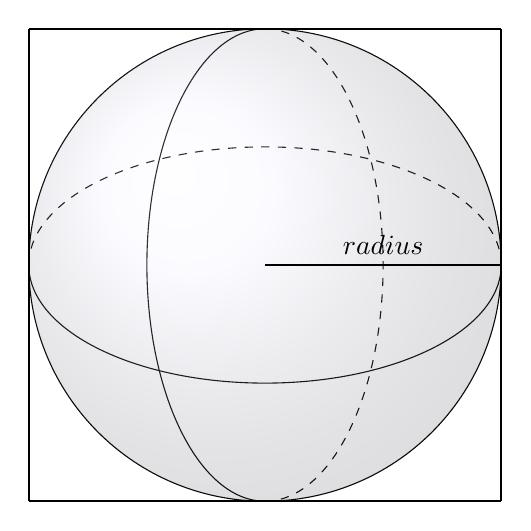
\begin{tikzpicture}[scale=3]
    \draw (-1,0) arc (180:360:1cm and 0.5cm);
    \draw[dashed] (-1,0) arc (180:0:1cm and 0.5cm);
    \draw (0,1) arc (90:270:0.5cm and 1cm);
    \draw[dashed] (0,1) arc (90:-90:0.5cm and 1cm);
    \draw (0,0) circle (1cm);
    \shade[ball color=blue!10!white,opacity=0.20] (0,0) circle (1cm);
    \draw[thick] (0,0) -- node[above]{$radius$} (1,0);
    %\draw[thick] (0,0) -- node[above]{$rd$} (-.7,-.7);
  
%\draw[blue,thick] (0,0,0) -- (0,2.75,0) -- (2.75,2.75,0) -- (2.75,0,0) -- cycle;
%\draw[blue,thick] (0,0,2.75) -- (0,2.75,2.75) -- (2.75,2.75,2.75) -- (2.75,0,2.75) -- cycle;
%
%%draw the edges of the cube
\draw[black,thick] (-1,-1) -- (1,-1);
\draw[black,thick] (-1,-1) -- (-1,1);
\draw[black,thick] (-1,1) -- (1,1);
\draw[black,thick] (1,-1) -- (1,1);
\end{tikzpicture}
\caption{A cuboid with minimal size layed around a sphere}
\label{tikz:CuboidSphere}
\end{center}
\end{figure}

To draw a cell as a sphere a new function had to be created. This function is named addSphereCell as it is displayed below. In the method all required points, the start- and end points as well as the centers, of all three axis are given in \SI{}{\micro\metre}. Thus, these points as well as the radius, which is also given to the function, and the steplength, i.e. the corner length of a voxel, are converted into the voxel unit. \newline
With all necessary points in the voxel unit it is now possible to iterate over all three axis and check for every voxel, if it is included in the sphere or not.

% With all required points it is now possible to iterate through every axis of the cuboid. I.e. first a position of the x-axis is selected, then a position at the y-axis is chosen and with these points every point of the z-axis will be checked if this coordinate is within the sphere or not. If all points of the z-axis are checked, then the position at the y-axis is increased and again all points at the z-axis are checked if they are in the sphere or not. If all points of the y-axis are checked then the position of the x-axis gets increased and the check starts again until every point of the cuboid is checked to be in the sphere or not.


\begin{lstlisting}[language=Python, caption = Function to draw a cell as a sphere. First all required points for the calculation are converted into the voxel unit. Then over each axis of the cuboid it is iterated. During these iterations for each voxel the distance to the center of the cuboid and sphere is calculated and then it is checked if the voxel is within the sphere or not. If the voxel is a part of the sphere it will be added to the sphere.]
    def _addSphereCell(self, typename, xPos, yPos, zPos, radius, steppable):
    
        cell = steppable.newCell(typename)
        xStart = self.execConfig.calcPixelFromMuMeter(xPos - radius)
        x0 = self.execConfig.calcPixelFromMuMeter(xPos)
        xEnd = self.execConfig.calcPixelFromMuMeter(xPos + radius)
        yStart = self.execConfig.calcPixelFromMuMeter(yPos - radius)
        y0 = self.execConfig.calcPixelFromMuMeter(yPos)
        yEnd = self.execConfig.calcPixelFromMuMeter(yPos + radius)
        zStart = self.execConfig.calcPixelFromMuMeter(zPos - radius)
        z0 = self.execConfig.calcPixelFromMuMeter(zPos)
        zEnd = self.execConfig.calcPixelFromMuMeter(zPos + radius)

        radiusPx = self.execConfig.calcFloatPixel(radius)
        stepLength = self.execConfig.calcFloatPixel(1)
        
        # loop over the center of each pixel to determine boundaries of the circle
        for xr in xrange(xStart, xEnd):
            for yr in xrange(yStart, yEnd):
                for zr in xrange(zStart, zEnd):
                    rd = sqrt(
                        ((xr+(((xr+stepLength) - xr)/2.)) - x0) ** 2 +
                        ((yr+(((yr+stepLength) - yr)/2.)) - y0) ** 2 +
                        ((zr+(((zr+stepLength) - zr)/2.)) - z0) ** 2)
                    if (rd <= radiusPx):
                        steppable.cellField[xr, yr, zr] = cell
                        
\end{lstlisting}

With this created function it is now possible to draw a cell as a sphere, as it is displayed at figure \textbf{xy}. \newline
To draw the cell as a sphere is the first step to have sphere cells in the simulation. Two major parts of the simulation are the growth and the mitosis of the simulation. In order that the cells are able to stay as a sphere it is required to adjust the volume and surface calculation as well.


\section{Growth of a sphere cell}
Since in the project morphogenesis of the urothelium is simulated, the drawn sphere cells are required to grow. \newline
In the simulation the current volume and surface of a cell is calculated by \ac{CC3D}. Every user is able to influence these values by setting the target volume and target surface and the proper multiplier, $\lambda_{vol}$ and $\lambda_{sur}$, for the specific part of the effective energy. Because the goal of the simulation is to minimize the effective energy, the cell will change the current volume and surface in the direction of the set target volume and target surface. 

To model the growth of a cell, the growth per day of the volume for the different cell types is set. Each calculation step the growth of one \ac{MCS} is calculated and applied, 500 calculations steps are one day. After the growth of the volume is calculated and set as new target volume of the specific cell, a new target surface depending on the target volume is calculated and set. \newline
In the program the target surface is calculated out of a real sphere and then multiplied by a factor.
Since the surface of a sphere of voxels is larger than the surface of a real sphere, it is necessary to find the correct factor, by which the surface of a sphere has to be multiplied, in order to calculate the surface of a sphere of voxels. 

For simplicity reasons, a first approximation of the factor is calculated in 2D. Thus, a circle and a square filled with pixels are used. An example therefor is displayed in figure \ref{img:CircleSquarePixels}. \newline
%Then, the calculated factor was used for the calculation of the deviation between the surface of a sphere and the surface of a sphere of voxels.
Figure \ref{img:ApproximationSQRT2} displays a approximation, with which it is possible to calculate the factor for the surface. 

\begin{figure}
	\center
	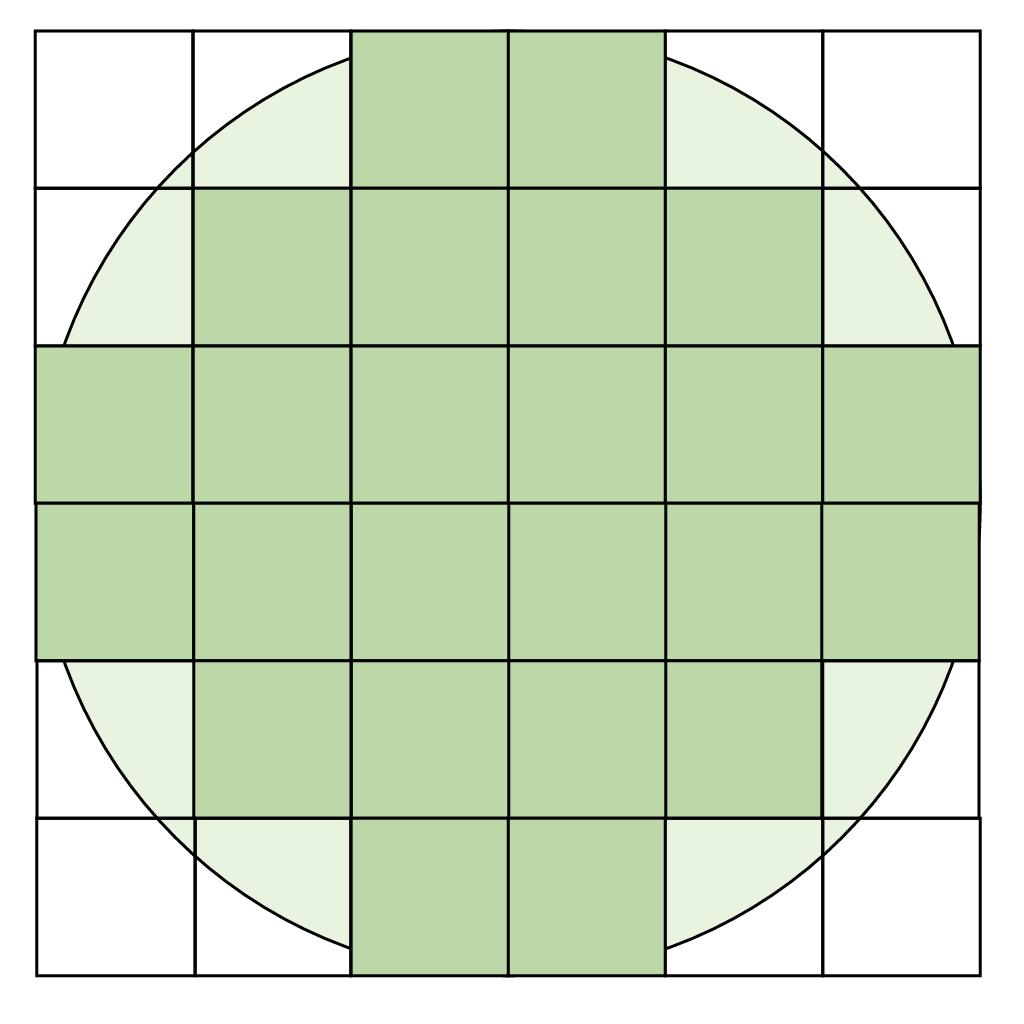
\includegraphics[scale=0.15]{figures/PixelCircleSquare.png}
	\caption{A circle in a possible pixel presentation. All small squares present pixels. The colored squares present the pixels, which are included in the pixel presentation of the circle.}
	\label{img:CircleSquarePixels}
\end{figure}

\begin{figure}
	\center
	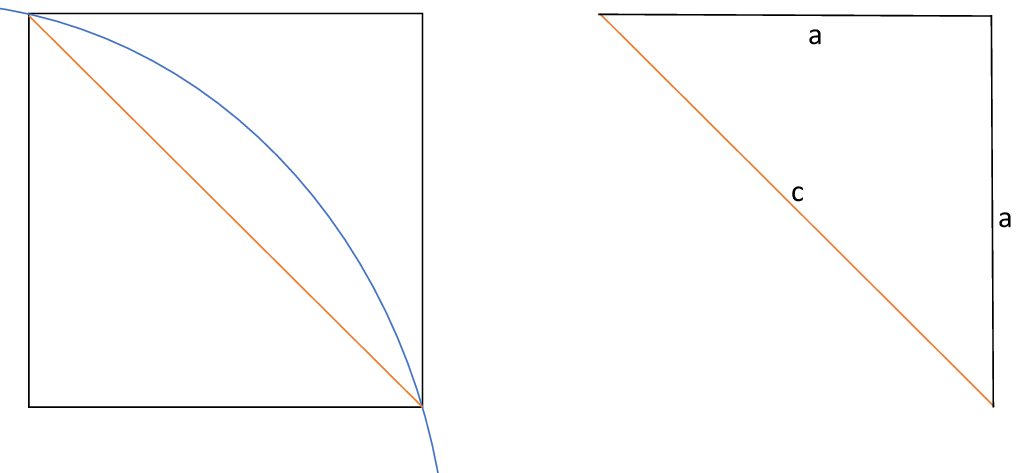
\includegraphics[scale=0.3]{figures/SurfaceApproximationSQRT2.png}
	\caption{The left part of the illustration displays a pixel at the surface, in which the circle goes through. The blue line represents the circle. As an approximation to the surface line a diagonal line in the square is drawn. With this diagonal line an isosceles, right ancular triangle appears and it is possible to calculate the additional surface of one pixel. This isosceles, right ancular triangle is displayed at the right side of this figure.}
	\label{img:ApproximationSQRT2}
\end{figure}

\begin{figure}
	\center
	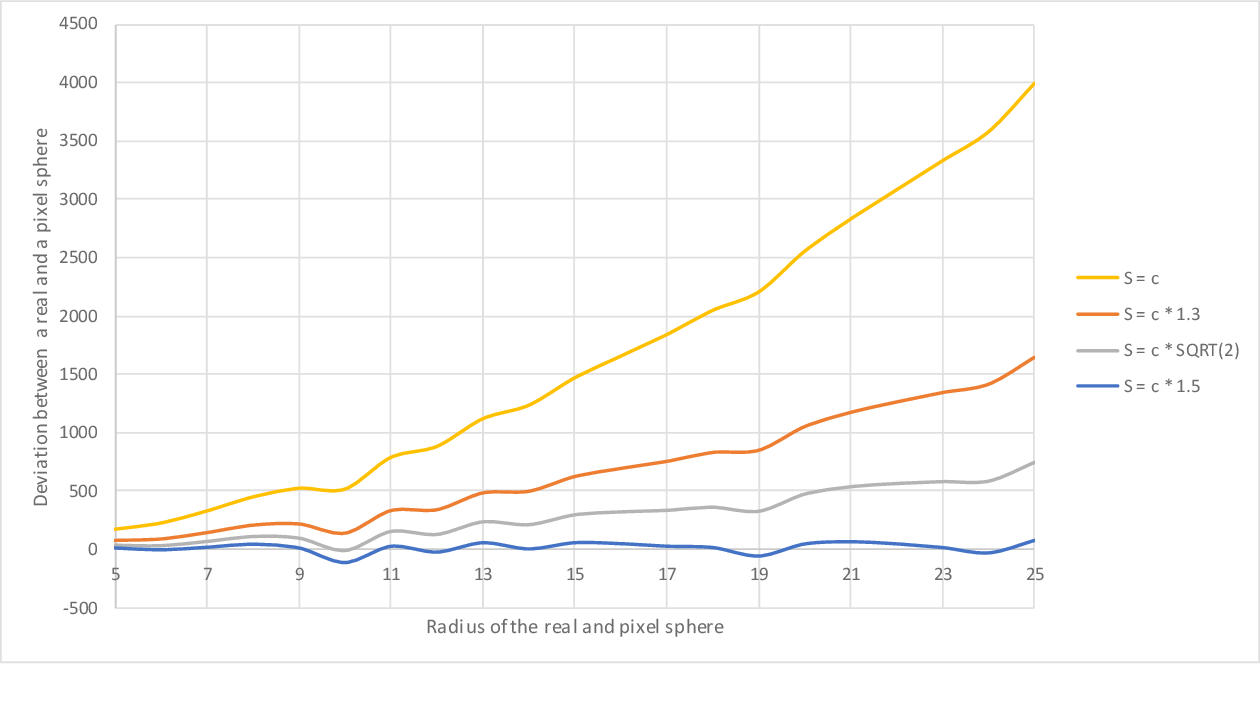
\includegraphics[scale=0.3]{figures/DeviationSphereToPixelSphere.png}
	\caption{Deviation between the surface of sphere of voxels and a real sphere. Each deviation is calculated with a different factor of the surface of the real sphere. $S$ refers to the surface of the sphere of voxels and $c$ refers to the surface of a real sphere. Thus, $c = 4 \cdot \pi \cdot r^{2}$. \newline
	At the x-axis the radius of the sphere and the sphere of voxels is displayed. At the y-axis the deviation between both surfaces is represented.}
	\label{img:DeviationSphere}
\end{figure}

In figure \ref{img:ApproximationSQRT2} the left square is considered as a pixel, it could be any pixel of the figure \ref{img:CircleSquarePixels} in which the circle goes through. Thus, the sides of the square are the same. The blue line represents the circle, in a way it could go through the pixel. An approximation is to insert a diagonal line. With this diagonal line an isosceles, right ancular triangle is created as it is displayed at the right side of figure \ref{img:ApproximationSQRT2}. \newline
The following formula provides a way to calculate the sides of the isosceles, right ancular triangle.
\begin{equation}\label{eq:IsoscelesRightAncularTriangle}
c^{2} = 2 \cdot a^{2}
\end{equation}
This formula can be used to calculate the side $a$, as it is displayed in the following equation.
\begin{equation}\label{eq:CornerSideAOfTriangle}
\begin{split}
a &= \sqrt{\dfrac{c^{2}}{2}} \\
a &= \dfrac{c \cdot \sqrt{2}}{2}
\end{split}
\end{equation}
Since the surface of a pixel has two corner sides, the equation to calculate the surface of a pixel sphere is
\begin{equation}\label{eq:PixelSurfaceCalculation}
\begin{split}
S &= 2a \\
S &= c \cdot \sqrt{2}
\end{split}
\end{equation}
This formula applies to all pixels, which are at the surface of the pixel sphere, $c$ is considered as the surface of the circle. Thus $c = \pi \cdot r^{2}$.

The calculated factor $\sqrt{2}$ was tested for a sphere surface. Because, this is an approximation to the surface of a pixel sphere, the tenth part beside this factor are also tested mathematically. As figure \ref{img:DeviationSphere} displays the  approximation with factor $\sqrt{2}$ still has some deviation. Almost no deviation between the surface of a sphere and a surface of a sphere of voxels is with a factor of $1.5$. Thus, this factor is applied for the calculation of the target surface. 

\section{Calculation of the volume and surface sites of a voxel sphere}
In order to calculate the voxel volume and the surface sites of a voxels sphere on our own, I created an algorithm for this problem. Otherwise for every measurement of the volume and surface of the sphere of voxels a new simulation in \ac{CC3D} had to be started. \newline
The algorithm requires the radius of the sphere, this radius has to be a whole number. For the tenths part between two whole numbers the result of the algorithm and \ac{CC3D} deviates.
Since a sphere and a cuboid are both symmetrical, it is possible to split both into 8 pieces. Doing so only one eighth of the of the cuboid has to be calculated in order to determine the volume and the surface of the sphere. \newline
To calculate which voxels are in the voxel sphere, the algorithm creates a x, z, y matrix. In the following calculations and decisions the center of each voxel is used. For every x,z voxel in the eighth of the cuboid the y constraint of the circle is calculated. Next, every voxel at the x,z coordinate is checked if the center of the voxel is within this constraint or not. Thus, every voxel at a x,z coordinate is checked if its center is within the sphere or not. This is repeated until every x,z coordinate of the eighth of the cuboid is calculated. Every time a voxel is within the sphere, it will be marked in the matrix.  \newline
To receive the volume of the voxel sphere all marked entries in the created matrix are count. Then, this result is mirrored for all three axis. Thus, the amount of marked voxels in the matrix is multiplied by 8, which equals to one multiply by 2 for each axis. Therefore $V=((Voxels \cdot 2) \cdot 2) \cdot 2$.
To receive the surface sites of the voxels at the surface, every marked entry is checked if the voxel at x+1, z+1 or the y+1 is either out of bounce, i.e. if it is outside the cuboid, or outside the sphere. Every of the three conditions is checked for every voxel within the surface. If one condition is true, the amount of surface sites is increased by 1. In the end the result, like the volume, has to multiplied by 8, in order to mirror the result for all three axis.


